%%%%%%%%%%%%%%%%%%%%%%%%%%%%%%%%%%%%%%%%%%%%%%%%%%%%%%%%%%%%%%%%%%%%%%%%%%%%%%%%%%%
% THE BEER-WARE LICENSE (Revision 42): %
% <r@twopi.eu> schrieb diese Datei. Solange Sie diesen Vermerk nicht entfernen, %
% können Sie mit dem Material machen, was Sie möchten. Wenn wir uns eines Tages %
% treffen und Sie denken, das Material ist es wert, können Sie mir dafür ein Bier %
% ausgeben. Robert Hemstedt %
%%%%%%%%%%%%%%%%%%%%%%%%%%%%%%%%%%%%%%%%%%%%%%%%%%%%%%%%%%%%%%%%%%%%%%%%%%%%%%%%%%%

\documentclass[12pt,a4paper]{article}
\usepackage[utf8x]{inputenc}
%\usepackage{ucs}
\usepackage[left=2.0cm, right=2.0cm, top=2.0cm, bottom=2.0cm]{geometry}
\usepackage{amsmath}
\usepackage{amsfonts}
\usepackage[ngerman]{babel}
\usepackage{bbm}
\usepackage{amssymb}
\usepackage[amsthm,thmmarks]{ntheorem}
%\usepackage{tabularx}
\usepackage[arrow, matrix, curve]{xy}
\usepackage{graphicx}
\usepackage{wrapfig}
\usepackage{color}
\usepackage{url}
% b) Lemma, Satz, Theorem usw.
\makeatletter
\renewtheoremstyle{plain}%
  {\item[\hskip\labelsep \theorem@headerfont ##1\ ##2:]}%
  {\item[\hskip\labelsep \theorem@headerfont ##1~##2~##3:]\mbox{}}
\makeatother

\theoremstyle{plain}
\newtheorem{Theorem}{Theorem}[section]
\newtheorem*{Satz}[Theorem]{Satz}
\newtheorem{Prop}[Theorem]{Proposition}
\newtheorem{Lemma}[Theorem]{Lemma}
\newtheorem{Korollar}[Theorem]{Korollar}
\newtheorem{Definition}[Theorem]{Definition}
\newtheorem*{Folgerung}[Theorem]{Folgerung}
\newtheorem*{Behauptung}[Theorem]{Behauptung}
\newtheorem{bez}[Theorem]{Bezeichnung}

\theorembodyfont{\upshape}
\newtheorem{Bemerkung}[Theorem]{Bemerkung}
\newtheorem{Beispiel}[Theorem]{Beispiel}

\newcommand{\herv}[1]{{\emph{\textbf{#1}}}}
\newcommand{\N}{\mathbb{N}}
\newcommand{\R}{\mathbb{R}}
\newcommand{\Z}{\mathbb{Z}}
\newcommand{\Q}{\mathbb{Q}}
\newcommand{\C}{\mathbb{C}}
\newcommand{\Ch}{\hat{\C}}
\newcommand{\cupdot}{\mathbin{\dot{\cup}}}

\def\presuper#1#2%
  {\mathop{}%
   \mathopen{\vphantom{#2}}^{#1}%
   \kern-\scriptspace%
   #2}

\numberwithin{equation}{section}

\newsavebox{\fmbox}
\newenvironment{fmpage}[1]
{\begin{lrbox}{\fmbox}\begin{minipage}{#1}}
{\end{minipage}\end{lrbox}\fbox{\usebox{\fmbox}}}

\linespread{1.05}
\author{Robert Hemstedt \\ \texttt{r@twopi.eu}}
\date{7. November 2014}
\title{Begleitmaterial Seminarvortrag Verzweigte Überlagerungen Riemannscher Flächen}
\begin{document}
\maketitle
Die schriftliche Ausarbeitung des Vortrags sowie dieses Begleitmaterial lassen sich in meinem \texttt{GitHub}-Repository \url{https://github.com/euklid/SeminarBranchedCovering} finden.
\section*{Endliche Automorphismengruppen der Zahlenkugel $\hat{\C}$}
\begin{Satz}
Jede nicht-zyklische, endliche Gruppe $G < \operatorname{Aut}(\Ch)$ der Ordnung $N$ hat genau drei Ausnahmeorbiten $\Sigma_1,\Sigma_2,\Sigma_3$. Für deren Mächtigkeiten $s_j :=\sharp\Sigma_j \geq 1$ und für die Ordnungen $n_j:=N/s_j$ der Standgruppen $G_a$ von $a\in \Sigma_j$ gibt es höchstens folgende Möglichkeiten: \begin{center}
\begin{tabular}{|c|c|c|c|c|c|c|c|} \hline
Typ & $N$ & $s_1$ & $s_2$ & $s_3$ & $n_1$ & $n_2$ & $n_3$ \\\hline
$q$-Dieder, $q\geq 2$ & $2q$ & $q$ & $q$ & $2$ & $2$ & $2$ & $q$ \\\hline
Tetraeder & $12$ & $6$ & $4$ & $4$ & $2$ & $3$ & $3$ \\\hline
Oktaeder & $24$ & $12$ & $8$ & $6$ & $2$ & $3$ & $4$ \\\hline
Ikosaeder & $60$ & $30$ & $20$ & $12$ & $2$ & $3$ & $5$ \\\hline
\end{tabular}
\end{center}
Sei $g_j$ ein erzeugendes Element der Standgruppe von $a_j \in \Sigma_j$. Dann wird $G$ von $\{g_1, g_2, g_3\}$ erzeugt. 
%Zwei Gruppen desselben Typs sind in $\operatorname{Aut}(\Ch)$ zueinander konjugiert.
\end{Satz}
\begin{figure}[h]
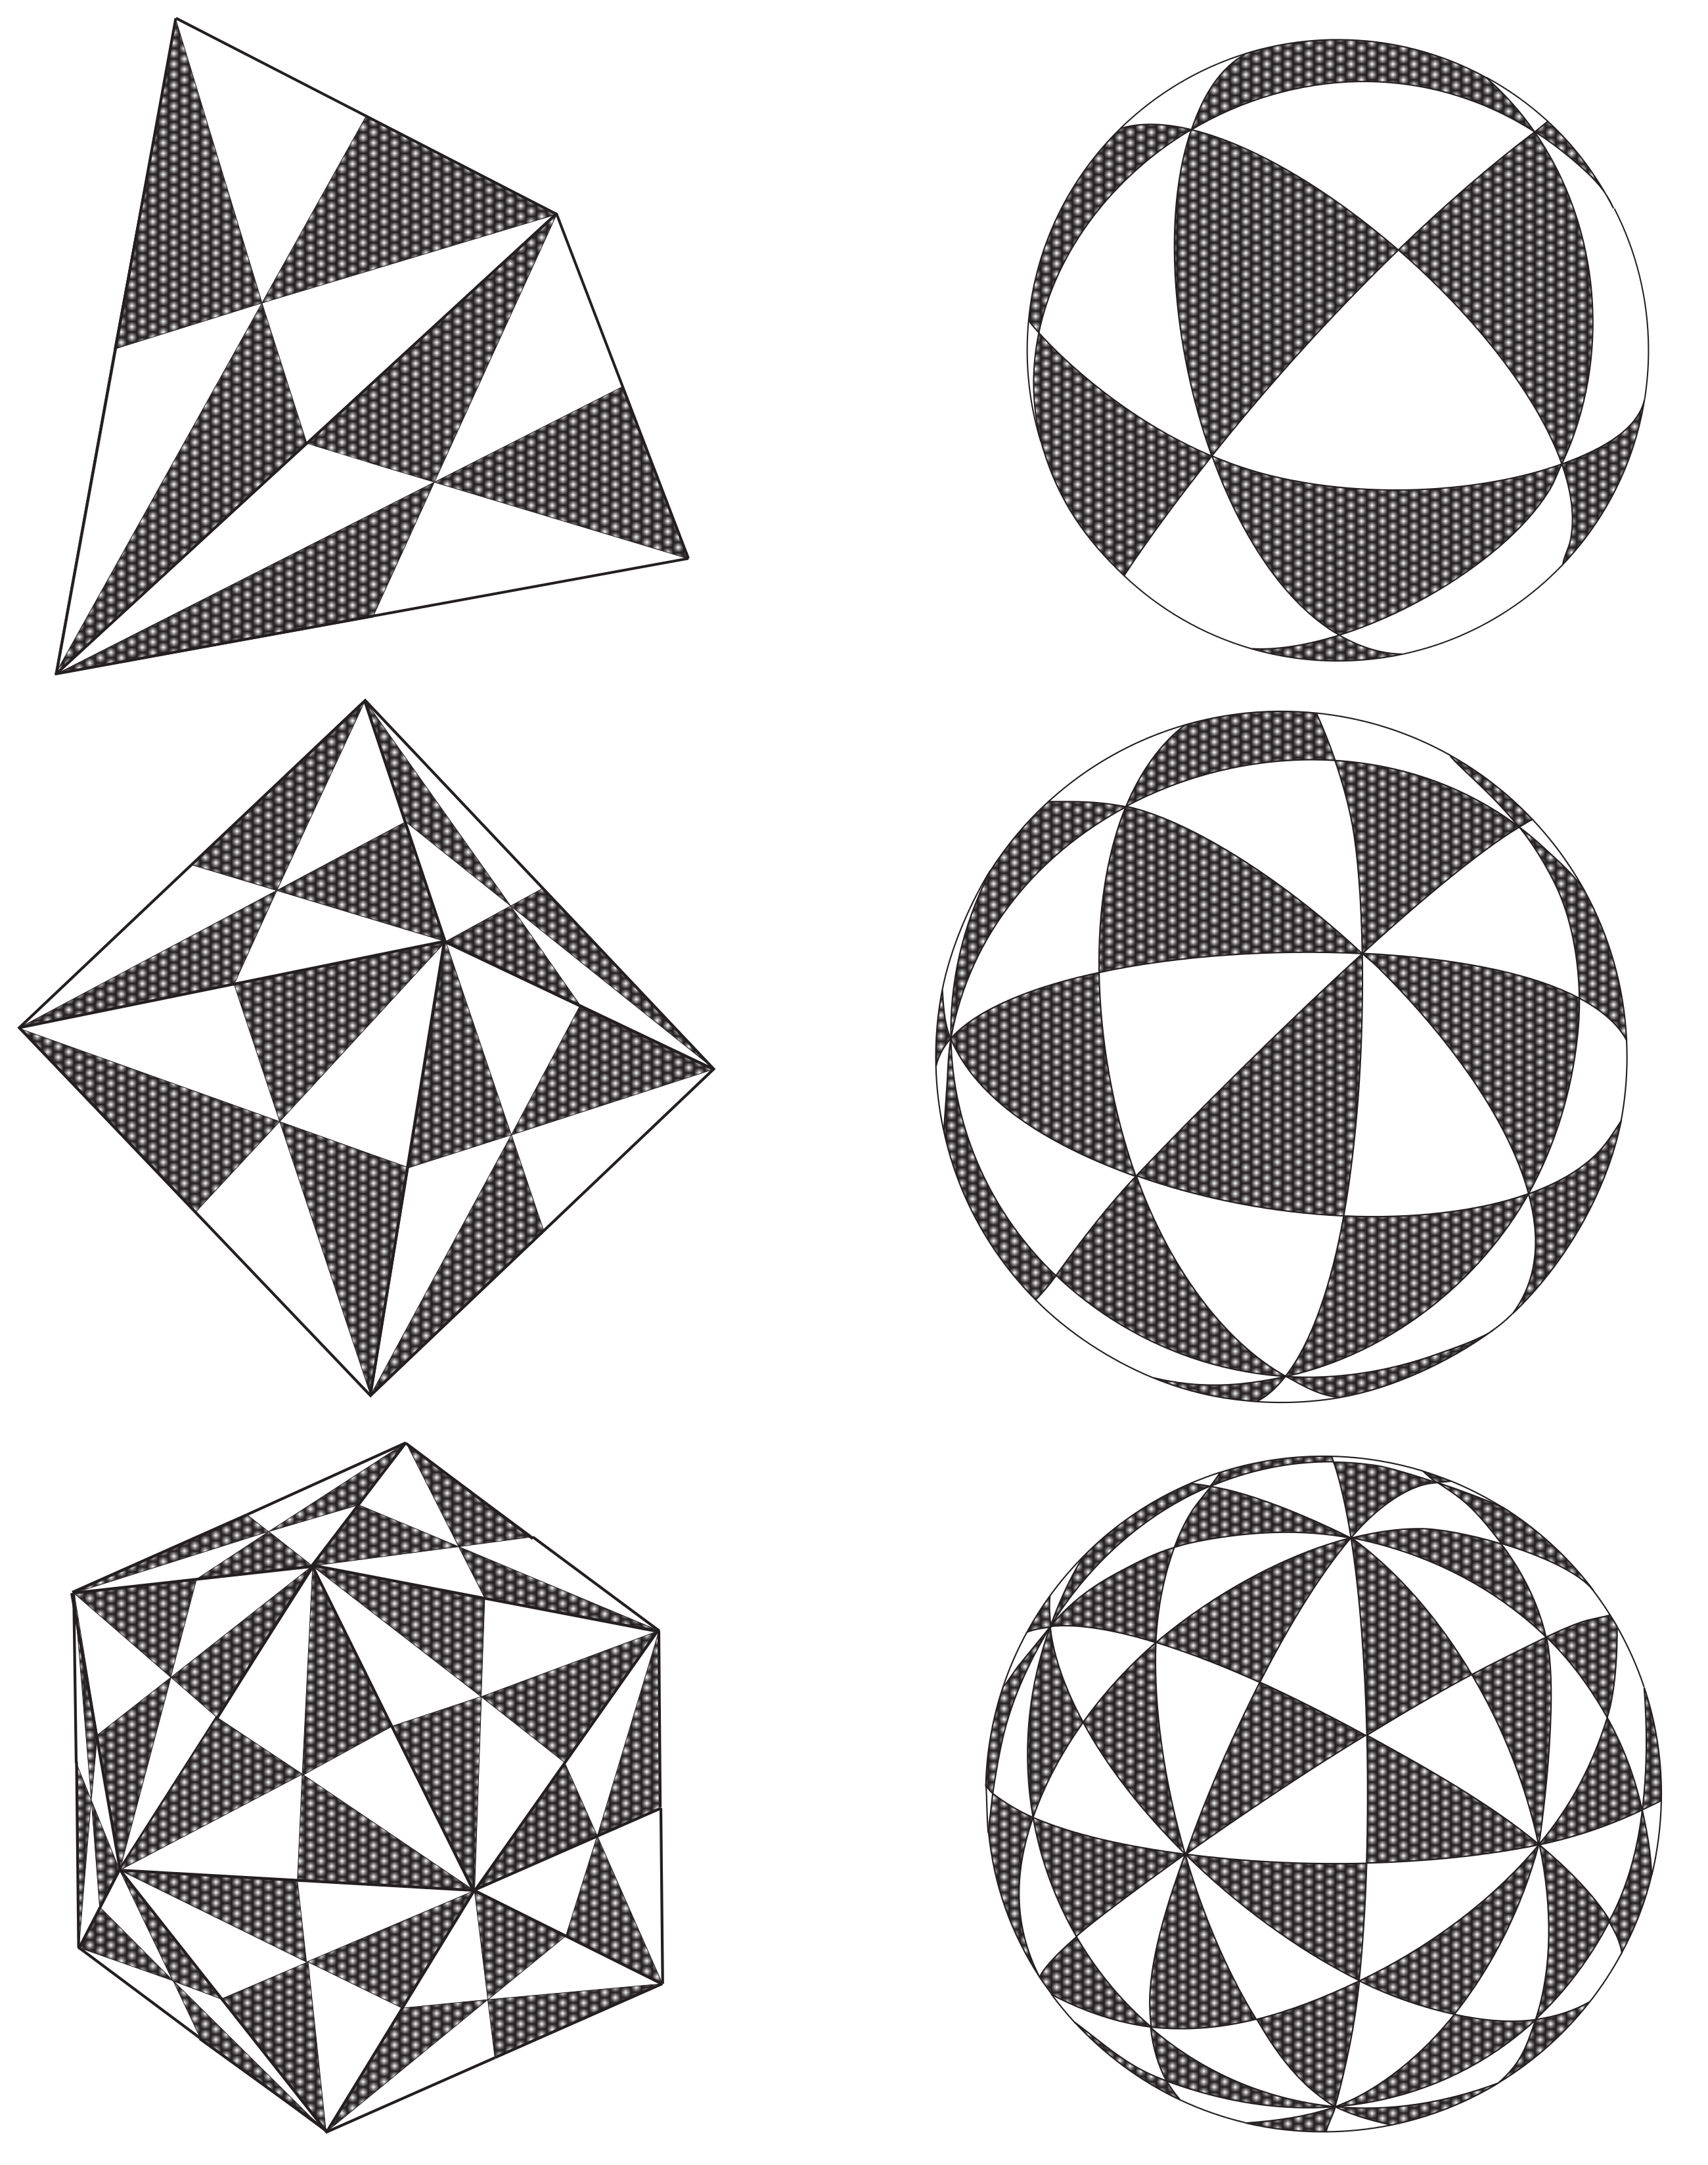
\includegraphics[width=0.8\textwidth]{polyeder.png}
\caption{Linksseitig Parkettierungen des Tetra-, Okta- und Ikosaeders mit Baryzentren jeder Seite. Rechtsseitg die Parkettierungen auf die $S^2$ mittels Radialprojektion übertragen.}
\end{figure}

\begin{figure} 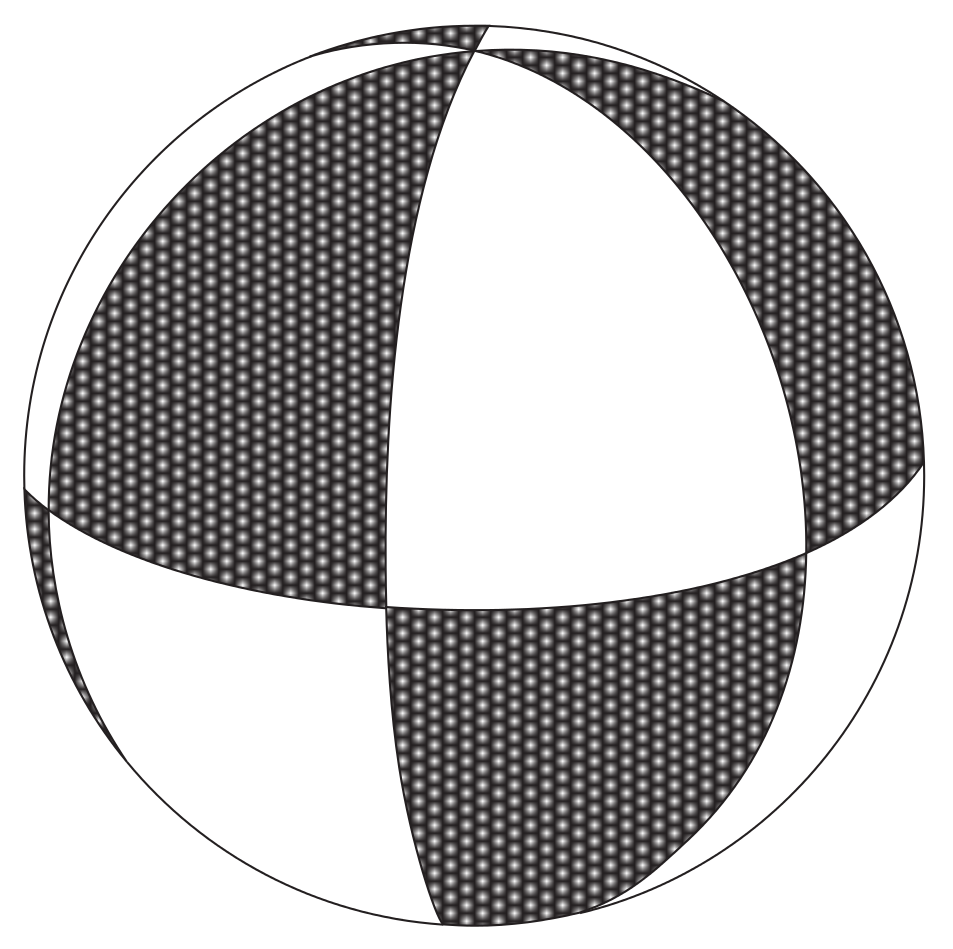
\includegraphics[width=0.5\textwidth]{Dieder.png}
\caption{$3$-Dieder-Parkettierung}
\end{figure}

\section*{Fortsetzung unverzweigter Überlagerungen}
\begin{Satz} Die unverzweigte Überlagerung $\eta: X\rightarrow Y\setminus B$ lässt sich genau dann zu einer Überlagerung $\hat{\eta}: \hat{X} \rightarrow Y$ fortsetzen, wenn jeder Punkt $b\in B$ Zentrum einer Scheibe $V$ ist, so dass für $V^\times:=V\setminus\{b\}$ und jede Komponente $U$ von $\eta^{-1}(V^\times)$ die Beschränkung $\eta|U: U\rightarrow V^\times$ endlich ist. Insbesondere existiert die Fortsetzung für jede endliche Abbildung $\eta$.
\end{Satz}
\begin{figure} \def\svgwidth{\textwidth} \input{KonstrVerzwUe.pdf_tex} \caption{Fortsetzung zur  verzweigten Überlagerung}\label{KVUe}
\end{figure}
\begin{proof}
Die Endlichkeitsbedingung an die Abbildung ist notwendig, wie wir an $\mathbb{H}\rightarrow \mathbb{E^\times}, z\mapsto e^{iz}$ gesehen haben. Konstruiere die Fortsetzung wie folgt:
\begin{itemize}
\item Wähle paarweise disjunkte Scheiben $V\subset Y$ um die Punkte in $b\in B$ und Karten $z:(V,b)\rightarrow (\mathbb{E},0)$.
\item Aus der Endlichkeitsbedingung folgt, dass es zu jeder Komponente $U$ von $\eta^{-1}(V^\times)$ einen Isomorphismus $h: U\rightarrow \mathbb{E}^\times$ mit $z\circ \eta|U = h^n$ gibt, $n$ abhängig von $U$.
\item Ergänze $U$ um Punkt $a_U$ zu $\hat{U}:=U\cupdot a_U$ und ergänze $h$ zur bij. Abbildung $h: (\hat{U},a_U) \rightarrow (\mathbb{E},0)$. Siehe Abb. \ref{KVUe}.
\item $A$ sei die Menge der zusätzlichen Punkte, dann definiere auf $\hat{X} = X \cupdot A$ die folgende Topologie: $W\subset \hat{X}$ offen, wenn $W\cap X \subset X$ offen in $X$ ist und für alle Komponenten $\hat{U}$ aus der Konstruktion die Bilder $h(W\cap \hat{U})\subset \mathbb{E}$ offen in $\mathbb{E}$ sind. Das macht $\hat{X}$ zu einem Hausdorff-Raum, so dass $A\subset \hat{X}$ lokal endlich ist.
\item Ergänze den holomorphen Atlas von $X$ um die Karten $h:\hat{U}\rightarrow \mathbb{E}$ der Konstruktion. Damit wird $\hat{X}$ zu einer Riemannschen Fläche.
\item Definiere $\hat{\eta}: \hat{X}\rightarrow Y$ durch $\hat{\eta}|X = \eta, \hat{\eta}(a_U)=b$ für $b$ Zentrum der Scheibe $V$, für die $U$ eine Komponente von $\eta^{-1}(V^\times)$ ist.
\item Aus der Konstruktion folgt, dass $\hat{\eta}:\hat{X}\rightarrow Y$ die Definition einer Überlagerung erfüllt und $\eta: X\rightarrow Y\setminus B$ fortsetzt.
\end{itemize}
\end{proof}
\section*{Quellen}
Riemannsche Flächen, Klaus Lamotke, 2., ergänzte und verbesserte Auflage, Springer, 2009.\\
Abbildung 1 und Abbildung 2 sind den Seiten 74 bzw. 73 entnommen.
\end{document}
